%*********************************************************************
%   APPENDIX SECTION: TEST SETUP
%   Supports Chapter 6 (and Chapter 7). Referenced from Section 6.1
%   as fig:test-setup.
%*********************************************************************
\FloatBarrier
\section{Test Setup}
\label{app:test-setup}

Every step test in Chapter~\ref{ch:thermalID} and every closed loop run in Chapter~\ref{ch:ClosedLoop} used the setup in Figure~\ref{fig:test-setup}. The chamber sat on the desk with water in the wells of a 96-well plate, and the sensor and heater wires passed through the cable gland. The electronics were left open on the desk next to it, since the wiring was changed between runs. The connections are listed in Section~\ref{app:wiring}.

\begin{figure}[H]
    \centering
    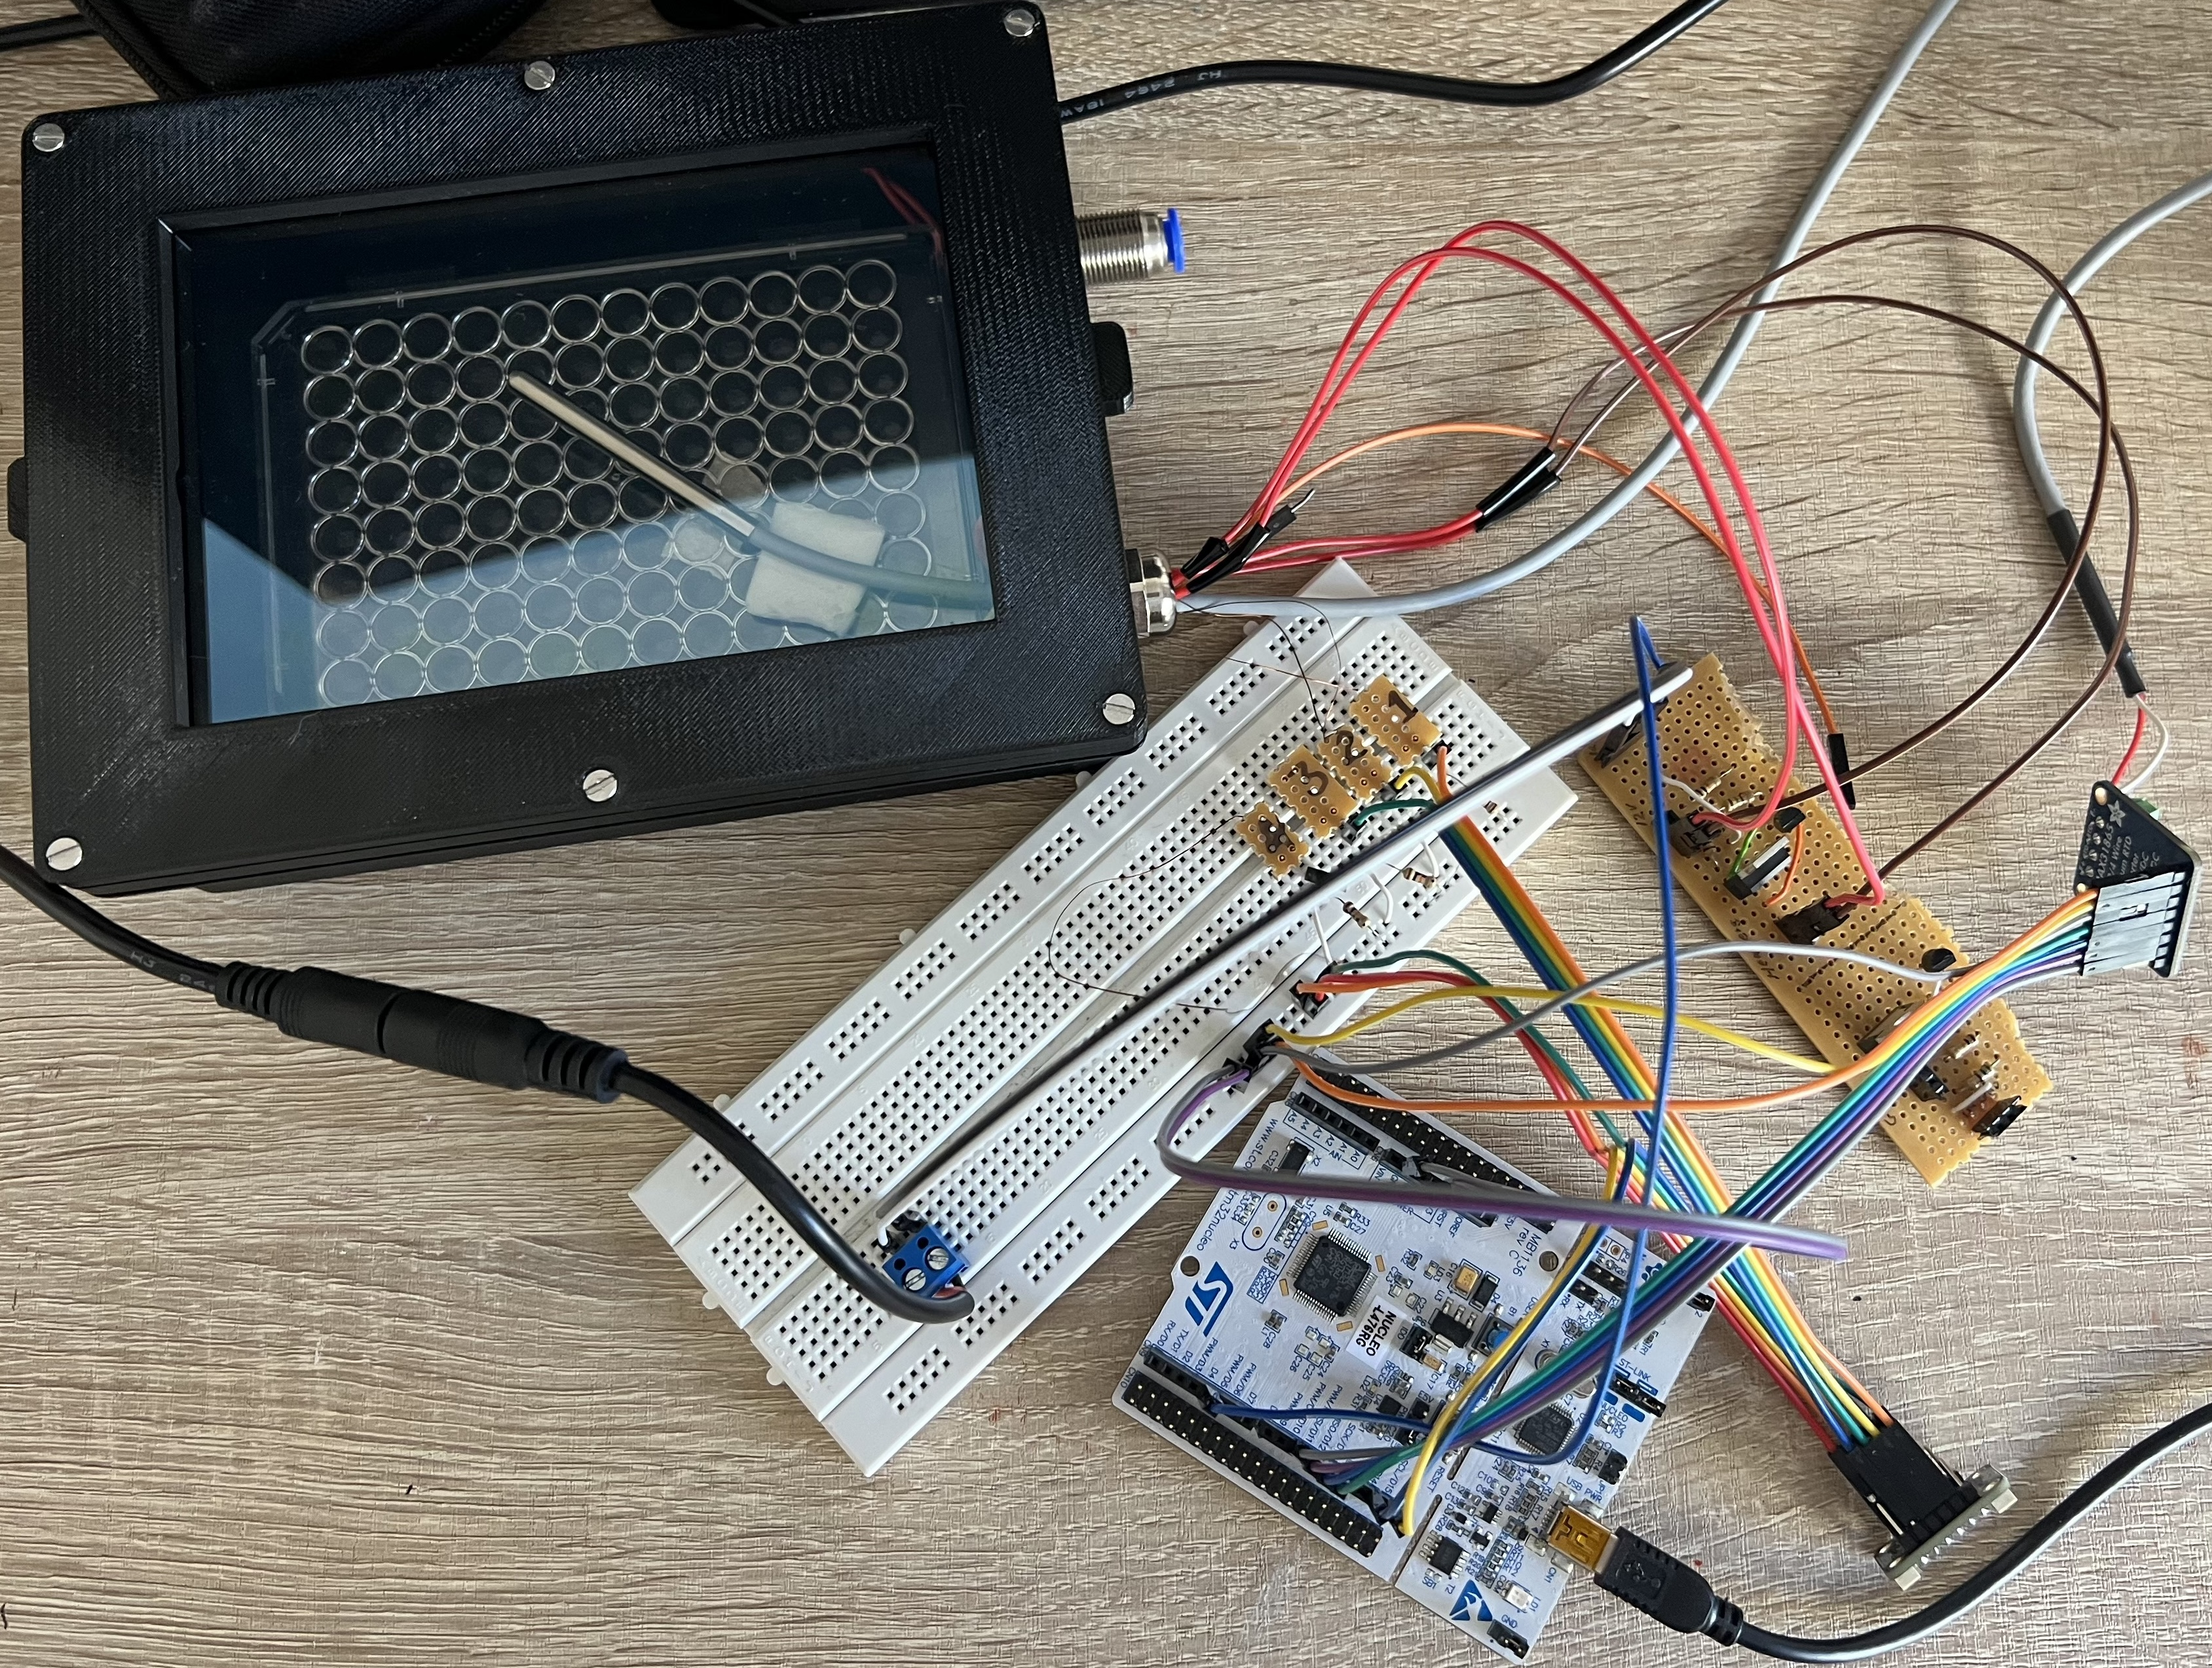
\includegraphics[width=0.82\textwidth]{figs/ch6/test-setup.jpeg}
    \caption[Test setup]{\textbf{The prototype during testing.} The chamber is closed with the ITO glass lid, with water in the wells of a 96-well plate inside. The PT1000 enters through the cable gland on the right-hand wall and sits in the air above the plate, with the gas fitting above it. On the bench are the STM32 Nucleo, the ADS1115 and MAX31865 converters, the heater drivers and the SCD30.}
    \label{fig:test-setup}
\end{figure}